\documentclass{article}

%\usepackage{corl_2023} % Use this for the initial submission.
\usepackage[final]{corl_2023} % Uncomment for the camera-ready ``final'' version.
%\usepackage[preprint]{corl_2023} % Uncomment for pre-prints (e.g., arxiv); This is like ``final'', but will remove the CORL footnote.

\usepackage{graphicx}
\usepackage{amssymb}
\usepackage{amsmath}
\usepackage{listings}
\usepackage{subcaption}
\usepackage{latexsym}
\usepackage{amsthm}
\usepackage{natbib}
\usepackage{listings}
\usepackage{hyperref} 

\title{Exercise 3 - Robot Learning Course}

% The \author macro works with any number of authors. There are two
% commands used to separate the names and addresses of multiple
% authors: \And and \AND.
%
% Using \And between authors leaves it to LaTeX to determine where to
% break the lines. Using \AND forces a line break at that point. So,
% if LaTeX puts 3 of 4 authors names on the first line, and the last
% on the second line, try using \AND instead of \And before the third
% author name.

% NOTE: authors will be visible only in the camera-ready and preprint versions (i.e., when using the option 'final' or 'preprint'). 
% 	For the initial submission the authors will be anonymized.

\author{
  Andrea Ongaro\\
	Computer Engineering\\
	Politecnico di Torino, Italy\\
	\texttt{s329706@studenti.polito.it} \\
  %% examples of more authors
  %% \And
  %% Coauthor \\
  %% Affiliation \\
  %% Address \\
  %% \texttt{email} \\
  %% \AND
  %% Coauthor \\
  %% Affiliation \\
  %% Address \\
  %% \texttt{email} \\
  %% \And
  %% Coauthor \\
  %% Affiliation \\
  %% Address \\
  %% \texttt{email} \\
  %% \And
  %% Coauthor \\
  %% Affiliation \\
  %% Address \\
  %% \texttt{email} \\
}


\begin{document}
\maketitle

%===============================================================================

\begin{abstract}
This article is the third in a series of three reports for the Reinforcement Learning laboratory course at Politecnico di Torino. This report is about policy gradient reinforcement learning algorithms within the OpenAI Gym environment, focusing on the CartPole problem. This process started implementing the naïve REINFORCE algorithm and then exploring more advanced Actor Critic methods like Proximal Policy Optimization (PPO) and Soft Actor Critic (SAC), also leveraging on the use of well-known
libraries such as Stable-Baselines3. Finally, you found the PPO is the best one to use in this context.

\end{abstract}

% Two or three meaningful keywords should be added here
\keywords{Reinforcement Learning, Robots, AI} 

%===============================================================================

\section{Introduction}
\subsection{The system - CartPole-v0}
CartPole-v0 system from OpenAI is part of the classic control environment. The starting code it's been provided by \href{https://www.polito.it/personale?p=andrea.protopapa}{Andrea Protopapa} in the course of Reinforcement Learning. Information about this system is sourced from the official documentation \cite{Cart_pole} and its GitHub repository. Below is the definition provided by the authors for CartPole-v0\\ \\
\textit{This environment corresponds to the version of the cart-pole problem described by Barto, Sutton, and Anderson in “Neuronlike Adaptive Elements That Can Solve Difficult Learning Control Problem”. A pole is attached by an un-actuated joint to a cart, which moves along a frictionless track. The pendulum is placed upright on the cart and the goal is to balance the pole by applying forces in the left and right direction on the cart.\citep{Cart_pole}}

For the following procedures, it's been used a modified version of the CartPole environment implemented in cp\_cont.py the standard CartPole uses discrete actions (applying force of either -10 or 10), while in this version it takes actions in the form of a single real number, which represents an arbitrary force value.
\begin{figure}[h]
	\centering
	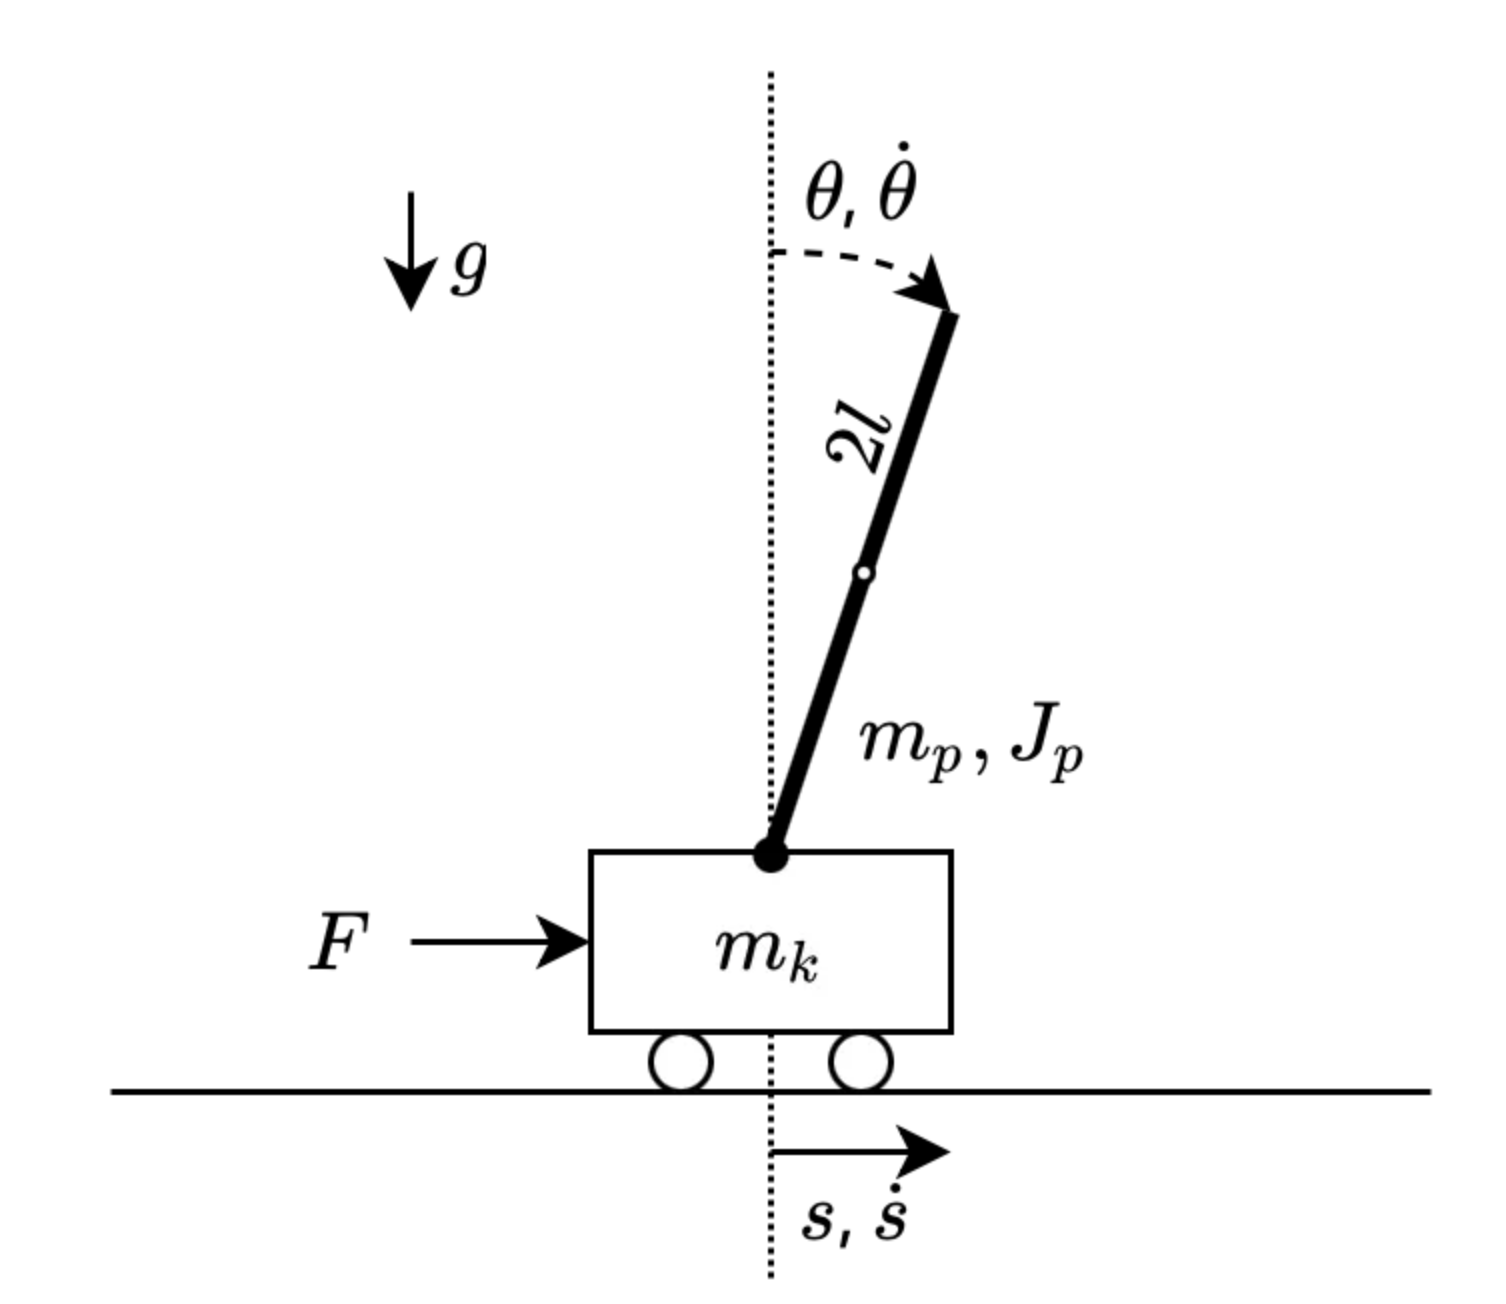
\includegraphics[width=0.5\linewidth]{../data/images/cart.png}
	\caption{Graphical explation about the whole system}
	\label{fig:plot1}
\end{figure}

\newpage

The observation is a four element vector: 
\begin{figure}[h]
	\centering
	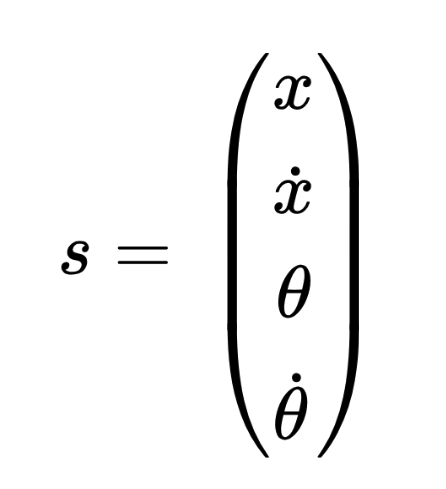
\includegraphics[width=0.2\linewidth]{../data/images/vector.png}
	\caption{Observation vector}
	\label{fig:plot2}
\end{figure}

where 
\begin{itemize}
	\item $x$: the position of the cart
	\item $\dot{x}$: the velocity, 
	\item $\theta$:  the angle of the pole
	\item $\dot{\theta}$: the angular velocity of the pole., 	
\end{itemize}

\subsection{REINFORCE algorithm}
REINFORCE is a policy-gradient method, a subset of policy-based approaches that focuses on directly optimizing the policy by iteratively adjusting its parameters through gradient ascent to maximize the objective function. This method estimates the weights of the optimal policy and updates them to improve performance over time.
%PROF

The REINFORCE algorithm is versatile and can be applied to various tasks, including complex control problems like robotics. However, it has notable limitations, such as high variance in gradient estimates and relatively slow convergence. To mitigate these challenges, several extensions and improvements have been developed, including the use of baseline functions to reduce variance, advantage estimation for more accurate updates, and trust region methods to ensure stable policy updates \cite{reinforce}.


\subsubsection{Baseline}
A baseline is a function used to adjust the return value during policy optimization. This adjustment can take various forms, ranging from sophisticated functions to, as demonstrated in this article, a simple constant value. In this context, a baseline is a value subtracted from the returns (or rewards) before calculating the gradient of the policy. Its primary purpose is to reduce the variance of gradient estimates, which can make learning more stable and efficient.

A constant baseline set to 20, which is simple to implement but may not account for the variability of rewards across different states, will be compared to two alternative approaches, both lacking a baseline: one where no adjustments are made to the rewards, and another where normalization is applied to the rewards..

\subsection{A good baseline}
%To choose a good baseline value, you need to understand what makes a baseline effective. The fundamental purpose of a baseline is to serve as a reference point against which you compare our actual returns. When you subtract this average from the actual returns, you get a much more meaningful signal. Actions that performed better than average get positive reinforcement, while those that performed worse than average get negative reinforcement, even if both gave positive raw rewards.
There are two ways to choose a good baseline, both with their advantanges and disadvantanges:

\subsubsection{Empirical Tuning Methods}
The empirical tuning approach involves setting the baseline based on actual observed returns, often using running averages or simple statistics. It's like setting a benchmark based on past performance. The main advantage of empirical tuning is its simplicity and stability.

\textbf{Whitening transformation} \\
Whitening transformation \cite{baseline_learning} standardizes the returns by not just centering them (subtracting the mean) but also decorrelating them and scaling to unit variance. This process "whitens" the data, meaning it transforms the returns to have zero mean, unit variance, and reduced correlations.

\subsubsection{Learned baseline}
This approach is more sophisticated and can be more effective, especially in complex environments. When you learn the baseline, you're essentially training a model to predict how well you expect to do in any given state. This prediction becomes our baseline.

You can make this even more sophisticated by using a state-dependent value function $V(s)$ as our baseline \cite{baseline}. This recognizes that different states naturally lead to different levels of reward. For example, in a game, being near a goal might naturally lead to higher rewards than being at the starting position. By using $V(s)$, we can better judge whether an action performed well given the specific situation.

\subsection{Training}
The baseline affects the training in different ways:

\subsubsection{Variance Reduction}
The primary effect is variance reduction. Without a baseline, the policy gradient would be influenced by the total magnitude of returns. The baseline helps prevent that misleading signals influence negatively the training (e.g. a poor strategy occasionally leads to a win) by comparing each outcome to what you typically expect.

\subsubsection{Learning Efficiency}
The baseline also improves learning efficiency \cite{baseline_learning}. Without it, the algorithm would waste time reinforcing actions that happened to occur during high-return episodes, even if those specific actions weren't responsible for the good outcome. The baseline helps distinguish between correlation and causation.

If the baseline is too high (much higher than typical returns), most actions will appear to perform poorly in comparison. This creates a situation where the policy receives mostly negative feedback, even for reasonably good actions. The learning process becomes inefficient because you're essentially telling the agent that "everything is bad," making it harder to identify truly beneficial actions.

Conversely, if our baseline is too low, most actions will seem better than the baseline. This creates the opposite problem - the agent gets positive reinforcement for many actions, even suboptimal ones.

\subsubsection{No Bias introduction}
A crucial property of baselines is that they must not introduce bias into the policy gradient estimates  \cite{baseline}. This means the baseline should not systematically shift our learning in any particular direction. The mathematical reason for this is that the baseline gets subtracted from our returns in a way that preserves the expected value of our gradient estimates.

\subsection{Real-world control problems}

\subsubsection{Risks with Unbounded Continuous Action Spaces and Reward Function}
In physical systems, a model with an unbounded continuous action space and a reward function introduces significant risks. Without bounded actions, the policy may propose extreme actions, potentially leading to system instability or even damage. Furthermore, with a simplistic survival-based reward structure (e.g., +1 for survival), the absence of penalties for extreme actions can mislead the agent into adopting overly aggressive policies that prioritize survival without considering safety constraints.

\textbf{How to mitigate these problems} \\
The most effective approach would be to modify the reward function. Here's some possible solutions to achieve the goal:
\begin{itemize}
	\item an action costs. 
	\item a soft barriers through exponentially increasing penalties. As actions get larger, the penalty grows rapidly, making extreme actions very costly but not impossible.
	%\item a learning approach where the model initially learns with smaller actions and gradually expands its action range as it demonstrates consistent, stable behavior. This helps develop more conservative policies naturally.
\end{itemize}

\subsubsection{Discrete action spaces}
Policy gradient methods can be used with discrete action spaces, but instead of sampling from a continuous distribution, the policy outputs a probability distribution over discrete actions, such as a Categorical distribution. This allows the log-probability of selected actions to be computed, enabling effective gradient updates. However, discrete action spaces come with their own challenges. Actions are sampled from the Categorical distribution, which, while straightforward, introduces randomness. Gradient estimation is typically well-defined through the log-probabilities, but ensuring sufficient exploration remains a key concern. Techniques like entropy regularization can help address this by encouraging the agent to explore a broader range of actions.

\newpage

\section{Actor Critic methods}
In REINFORCE, the goal is to increase the probability of actions in a trajectory in proportion to the magnitude of the return. However, due to the stochastic nature of both the environment (random events occurring during an episode) and the policy, trajectories starting from the same initial state can lead to vastly different returns. This variability introduces high variance into the gradient estimates, making it challenging to achieve stable learning. As a result, returns for the same starting state can fluctuate significantly across episodes \cite{variance}.

The Actor-Critic method addresses some of these challenges by combining Policy-Based and Value-Based approaches. It relies on two function approximations: the Actor, which parameterizes the policy function, and the Critic, which parameterizes the value function. At each timestep, the current state is obtained from the environment and passed as input to both the Actor and Critic.

To further stabilize learning, the method can use the Advantage function as the Critic instead of the Action-Value function. The Advantage function measures the relative benefit of taking a specific action compared to the average reward expected at that state. Essentially, it quantifies the “extra” reward obtained by taking a particular action at a given state compared to the mean reward for that state, making it a more effective guide for policy updates \cite{actor_critic}.

\subsection{PPO \& SAC}
Algorithms designed for continuous action spaces, such as PPO and SAC, must effectively handle a continuous range of values for each action dimension, enabling them to manage the fine-grained control required in such environments.

\textbf{Proximal Policy Optimization (PPO)} is an on-policy algorithm that employs a stochastic policy, typically modeled with a Gaussian distribution, to generate continuous actions. This setup allows PPO to excel in continuous action environments by balancing exploration and exploitation. PPO is known for its faster convergence and stability, making it well-suited for tasks involving continuous state and action spaces. 

To avoid destabilizing training with overly large policy updates, PPO introduces a clipping mechanism that restricts the probability ratio between the updated and old policies to ensure gradual changes. Additionally, PPO updates the policy iteratively over multiple epochs and mini-batches, promoting efficient and stable learning. Avoiding large policy updates is crucial for two reasons: empirically, smaller updates are more likely to converge to an optimal solution, and taking overly large steps risks “falling off the cliff,” leading to a poor policy that may be challenging or impossible to recover from. \cite{ppo_sac}

\textbf{Soft Actor-Critic (SAC)} is an off-policy algorithm tailored for continuous action spaces. Like PPO, it uses a stochastic policy modeled by a Gaussian distribution but distinguishes itself through entropy regularization, which enhances exploration by encouraging the selection of diverse actions. This feature helps SAC avoid premature convergence to suboptimal solutions, often resulting in superior performance in continuous action environments. SAC’s objective is to maximize both the expected return and the entropy of the policy. The entropy regularization term, added to the objective function, measures the randomness of the policy and ensures robust exploration. While SAC offers better exploration and resilience against convergence issues, it generally requires more computational resources and longer training times than PPO. \cite{ppo_sac}

\newpage
\section{Experiments}
This section presents a series of tests applying various methods to address the same problem: stabilizing the pole over the episodes. Each approach is evaluated based on the return value over the training period, highlighting their respective strengths and limitations. All the trainings was completed with this configuration:
\begin{itemize}
	\item MacBook Pro M1
	\item Python: 3.8.20
	\item OS: macOS-15.2-arm64-arm-64bit root:xnu-11215.61.5~2/RELEASE\_ARM64\_T6000
	\item Stable-Baselines3: 1.6.2
	\item PyTorch: 2.1.0
\end{itemize}

\subsection{REINFORCE}

\subsubsection{REINFORCE without baseline}
The first method explored is the use of REINFORCE without a baseline. As demonstrated by the graph (Figure \ref{fig:plot3}), this approach is not suitable for solving the given task, as the agent fails to exhibit clear convergence to an optimal policy. 
The reward curve is noisy, indicating high variability in the rewards as explained earlier while the 100-episode average curve shows that learning progresses is nearly inenexisting, with periods of by plateaus and declines. Overall, the agent struggles to make consistent progress achieving a final bad result.

\begin{figure}[h]
	\centering
	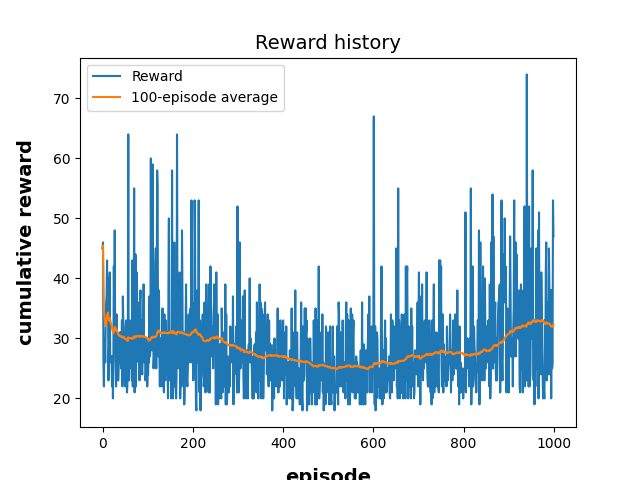
\includegraphics[width=0.5\linewidth]{../data/plot/reward_history_ContinuousCartPole-v0_0_basic.png}
	\caption{Reward history - Basic REINFORCE no baseline}
	\label{fig:plot3}
\end{figure}

\subsubsection{REINFORCE with a constant baseline $b = 20$}
In contrast, the constant baseline case (Figure \ref{fig:plot4}) shows different behavior.
The agent starts with higher performance (around 25-50) and demonstrates a more gradual but consistent improvement over time. This plot reveals that the agent actually achieves some of its best performance in the final episodes, with raw rewards reaching around 200.

%Average test reward: 158.4 episode length: 158.4
\begin{figure}[h]
	\centering
	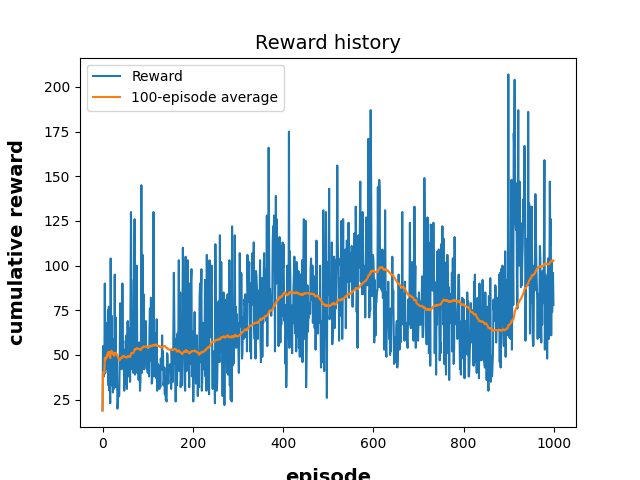
\includegraphics[width=0.5\linewidth]{../data/plot/reward_history_ContinuousCartPole-v0_0_constant_baseline.png}
	\caption{Reward history - Basic REINFORCE with b = 20}
	\label{fig:plot4}
\end{figure}

\newpage

\subsubsection{REINFORCE with normalized rewards}
A normalized rewards fixes them by centering them around their mean and scaling them by their standard deviation. It helps stabilize training by reducing the range and variance of the rewards, which is especially useful when raw rewards vary significantly:

\centering
$\text{Normalized rewards} = \frac{R - \text{mean}(R)}{\text{std}(R) + \epsilon}$

\flushleft

where  $\epsilon$  is a small constant to avoid division by zero.

In this case, you see a generally upward trend in the 100-episode average (orange line), starting around 40-50 and gradually improving to around 90-100 by the end of training. This suggests that normalization is helping the agent make steady progress over time.

Starting from around 40-50 baseline, the agent's performance improves steadily in the first 400 episodes, reaching its peak performance with the 100-episode moving average hitting approximately 100. After this peak, there's a noticeable decline in performance before it stabilizes at a lower level around episode 600. The raw rewards  show significant volatility throughout, with some exceptional peaks reaching up to 225, 

%Average test reward: 193.6 episode length: 193.6 %Average test reward: 134.6 episode length: 134.6 %Average test reward: 186.0 episode length: 186.0
\begin{figure}[h]
	\centering
	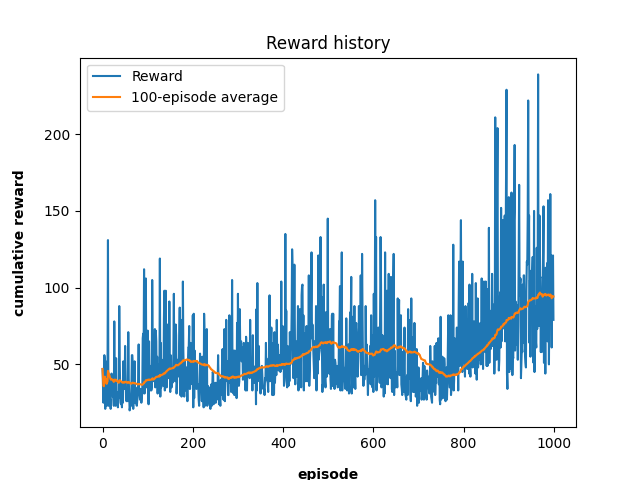
\includegraphics[width=0.5\linewidth]{../data/plot/reward_history_ContinuousCartPole-v0_0_normalized.png}
	\caption{Reward history - Basic REINFORCE with discounted rewards normalized to zero mean and unit variance,}
	\label{fig:plot5}
\end{figure}

\newpage

\subsubsection{Results}
The training times for the training without a baseline required an average time of 5.25 seconds with average reward of 31.15, the variant using a constant baseline increased the average training time to 11.01 seconds with average reward of 102.38 and the last method took about 10.27 seconds with average reward of 62.19.

During testing, the results closely resemble those from the training phase. The basic method, which lacks any enhancements, performs the worst with an average reward of 27. The best performance is achieved by the constant baseline method, reaching an average reward of 132.9, followed by the normalized rewards method with an average reward of 68.



\subsubsection{Variability}
As shown in Figures \ref{fig:plot10}, \ref{fig:plot11}, and \ref{fig:plot12}, the REINFORCE algorithm exhibits significant variability. This variability can lead to different rewards across individual runs, making its performance less predictable, even if, generally speaking, runs don't go too much outside the expected range of value.

%The basic REINFORCE without a baseline is like trying to learn a skill without any reference point. Sometimes you might get lucky and find a good approach quickly, but more often, you'll struggle with inconsistent feedback.

%Adding a constant baseline is like having a fixed reference point  This helps provide some consistency in learning, but it's not perfect because that fixed reference point might not always be appropriate. This is why we often see better initial learning compared to no baseline, but still significant variation between runs and potential performance collapses.

%The normalized rewards approach is like having an adaptive reference point that changes based on your recent performance. This typically provides the most stable learning progress.This is why even the most stable version (normalized rewards) still shows variation between runs.

\begin{figure}[h]
	\centering
	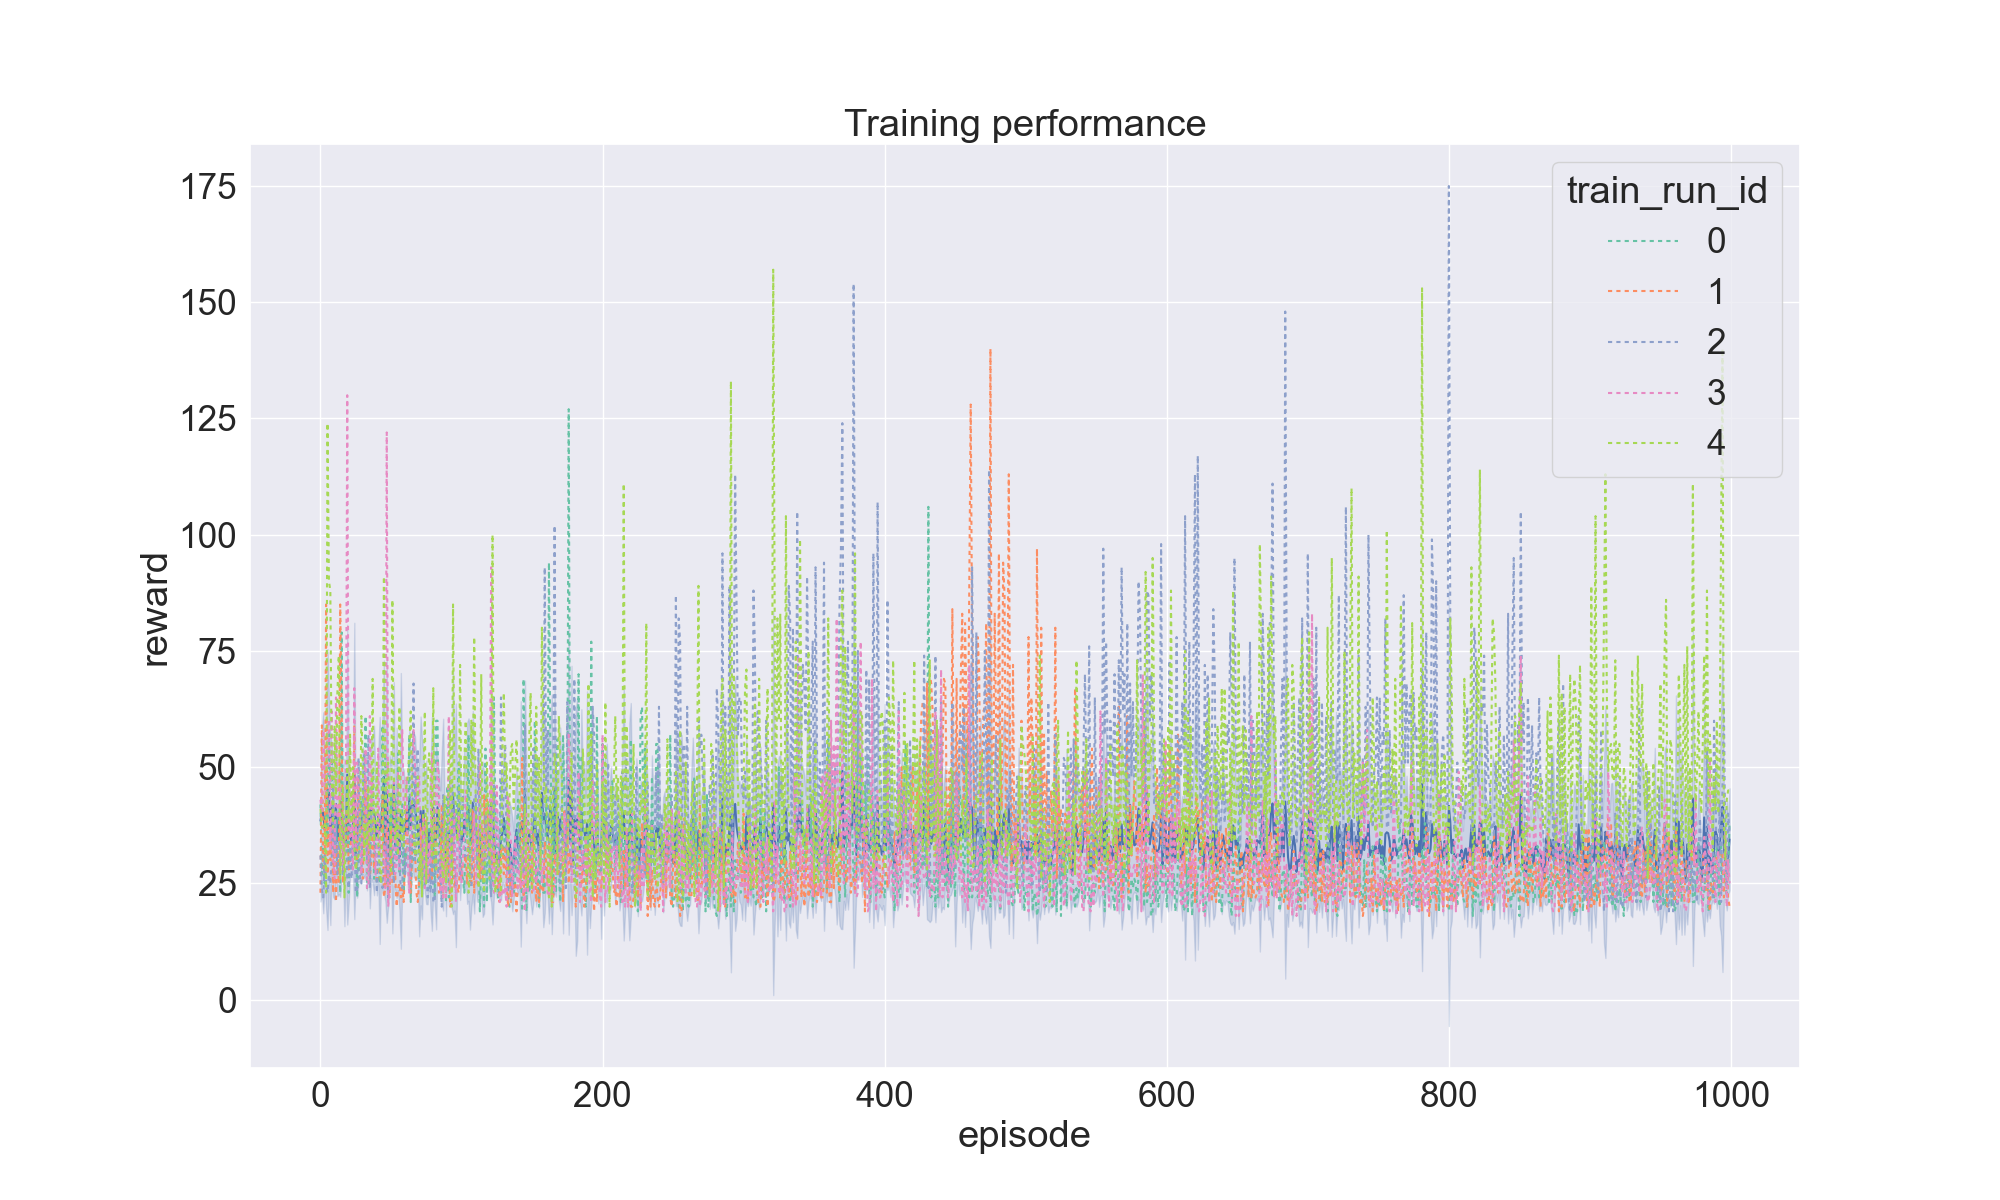
\includegraphics[width=0.9\linewidth]{../data/plot/training_multiple_basic.png}
	\caption{Mutliple run Reward history - REINFORCE with no baseline}
	\label{fig:plot10}
\end{figure}

\begin{figure}[h]
	\centering
	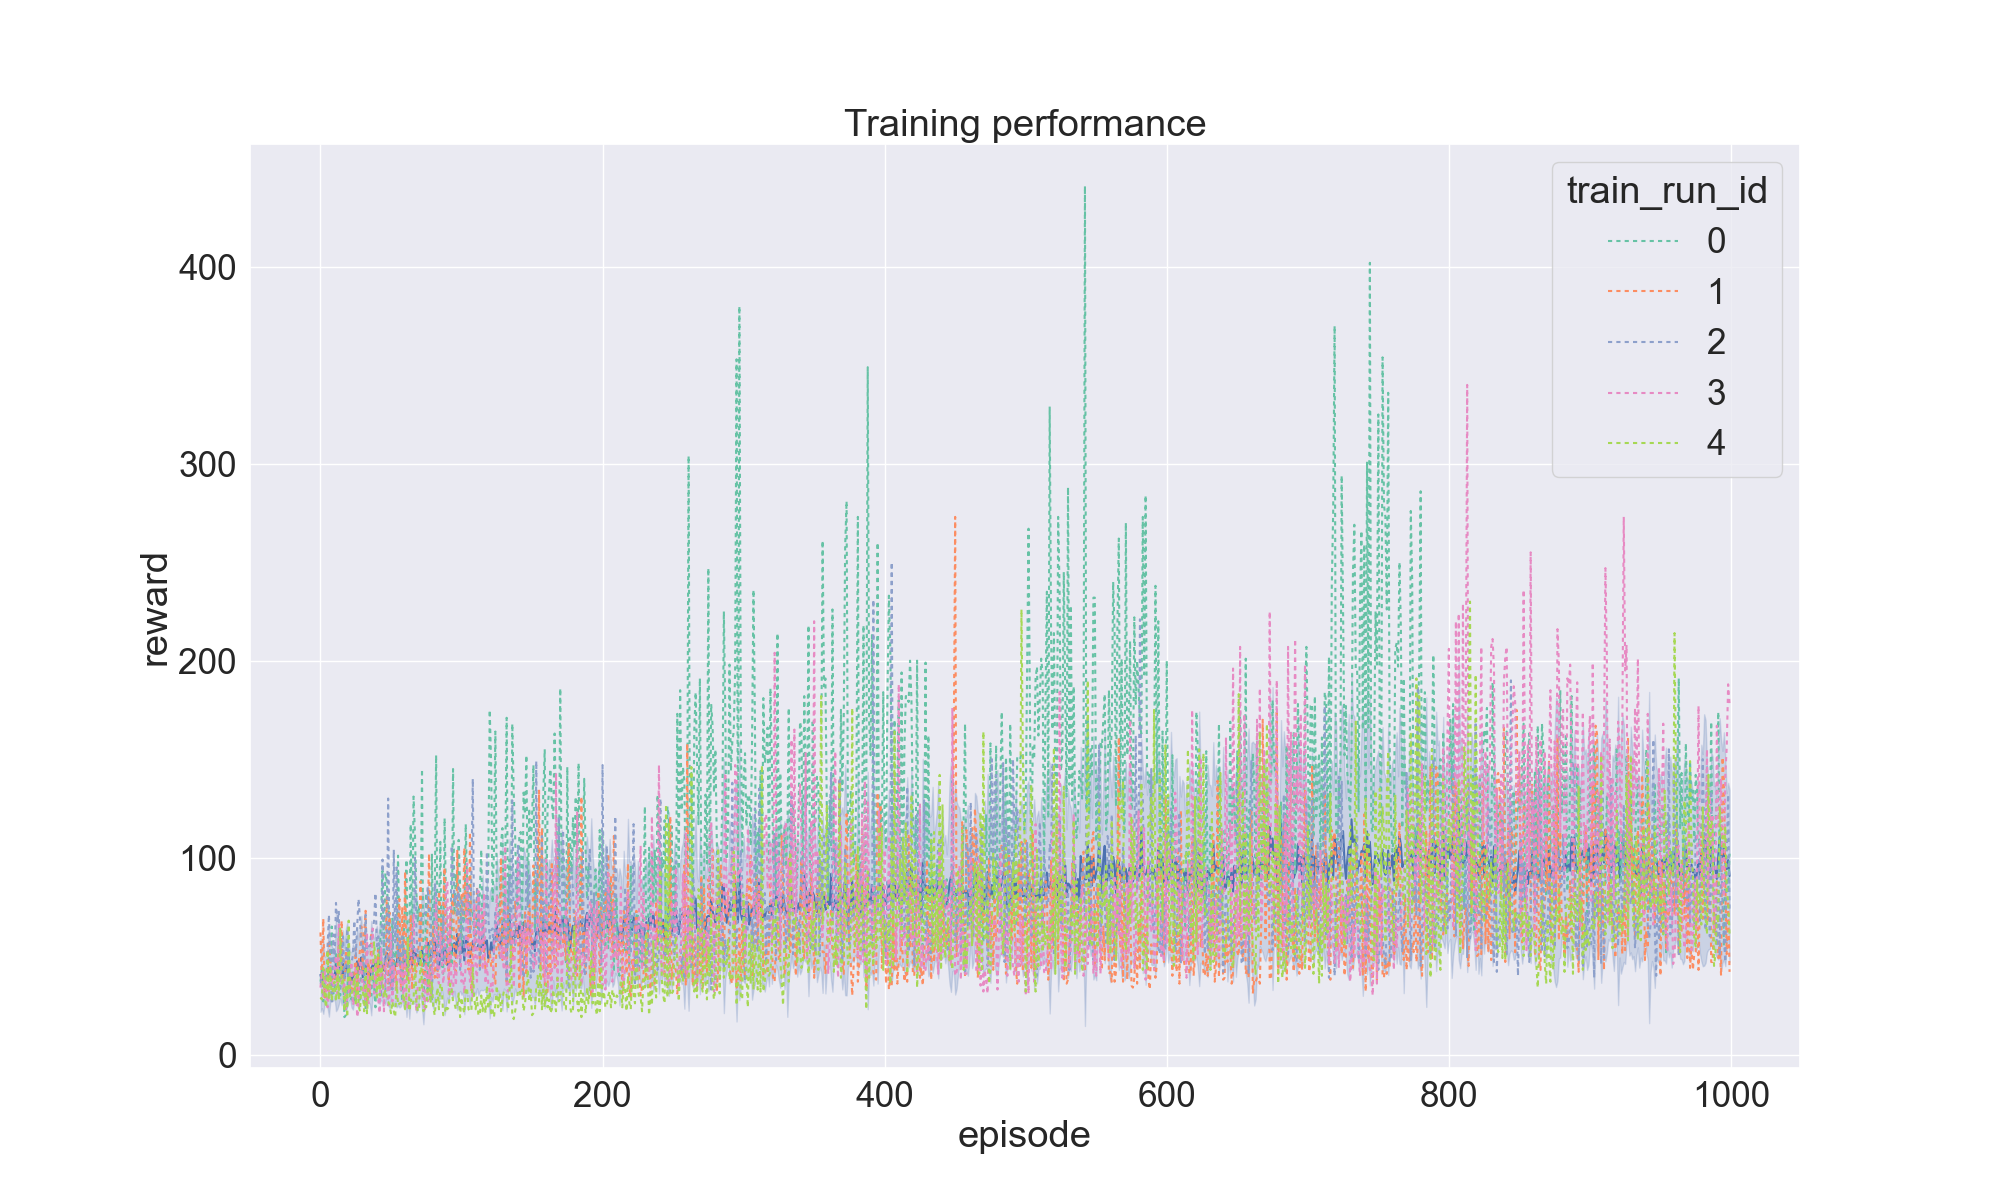
\includegraphics[width=0.9\linewidth]{../data/plot/training_multiple_constant_baseline.png}
	\caption{Mutliple run Reward history - REINFORCE with b = 20}
	\label{fig:plot11}
\end{figure}

\begin{figure}[h]
	\centering
	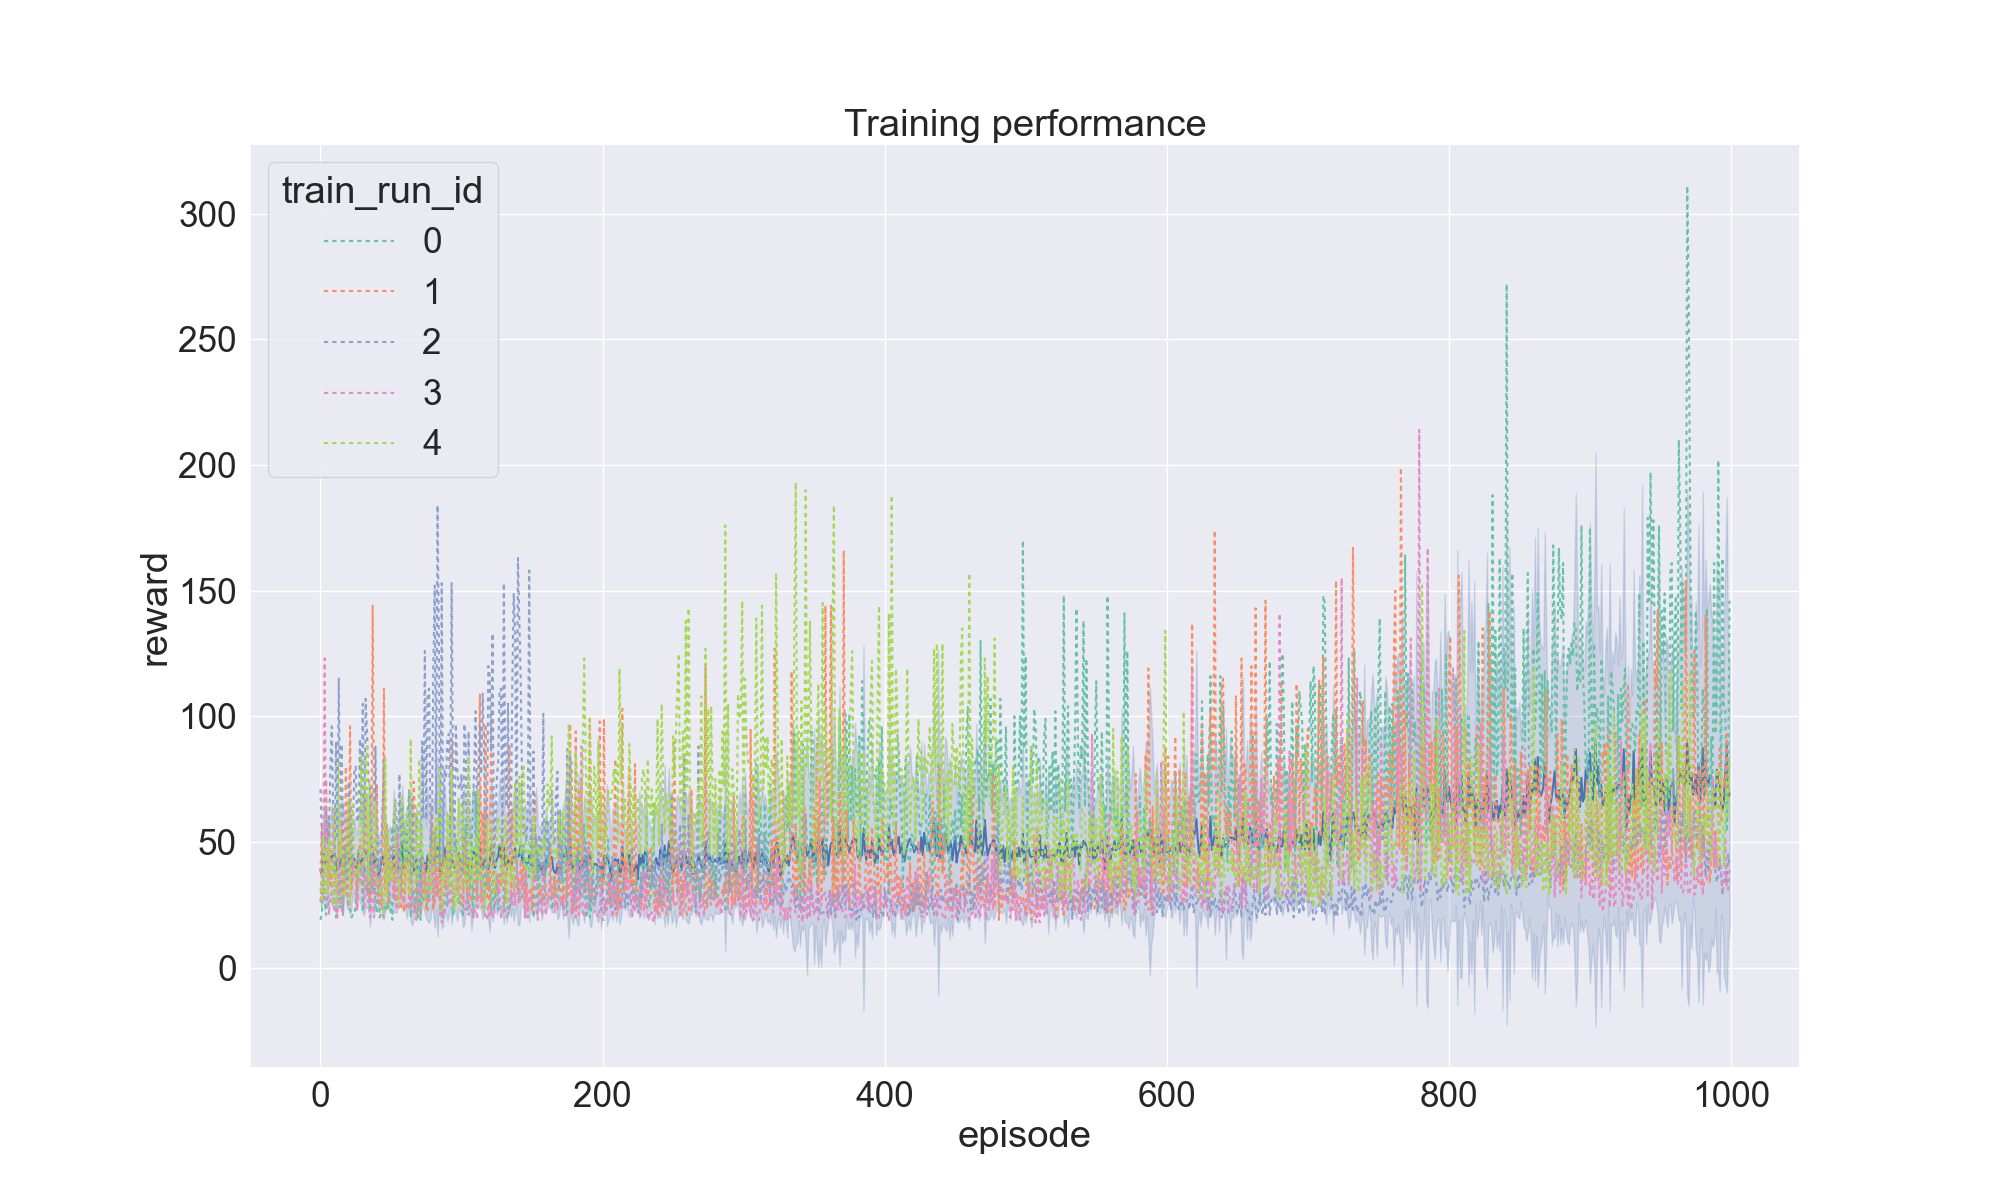
\includegraphics[width=0.9\linewidth]{../data/plot/training_multiple_normalized.png}
	\caption{Mutliple run Reward history - Normalized rewards}
	\label{fig:plot12}
\end{figure}

In Figure \ref{fig:plot15}, the graph illustrates the reward values across 30 runs, providing a clearer comparison of their variability and trends.

\begin{figure}[h]
	\centering
	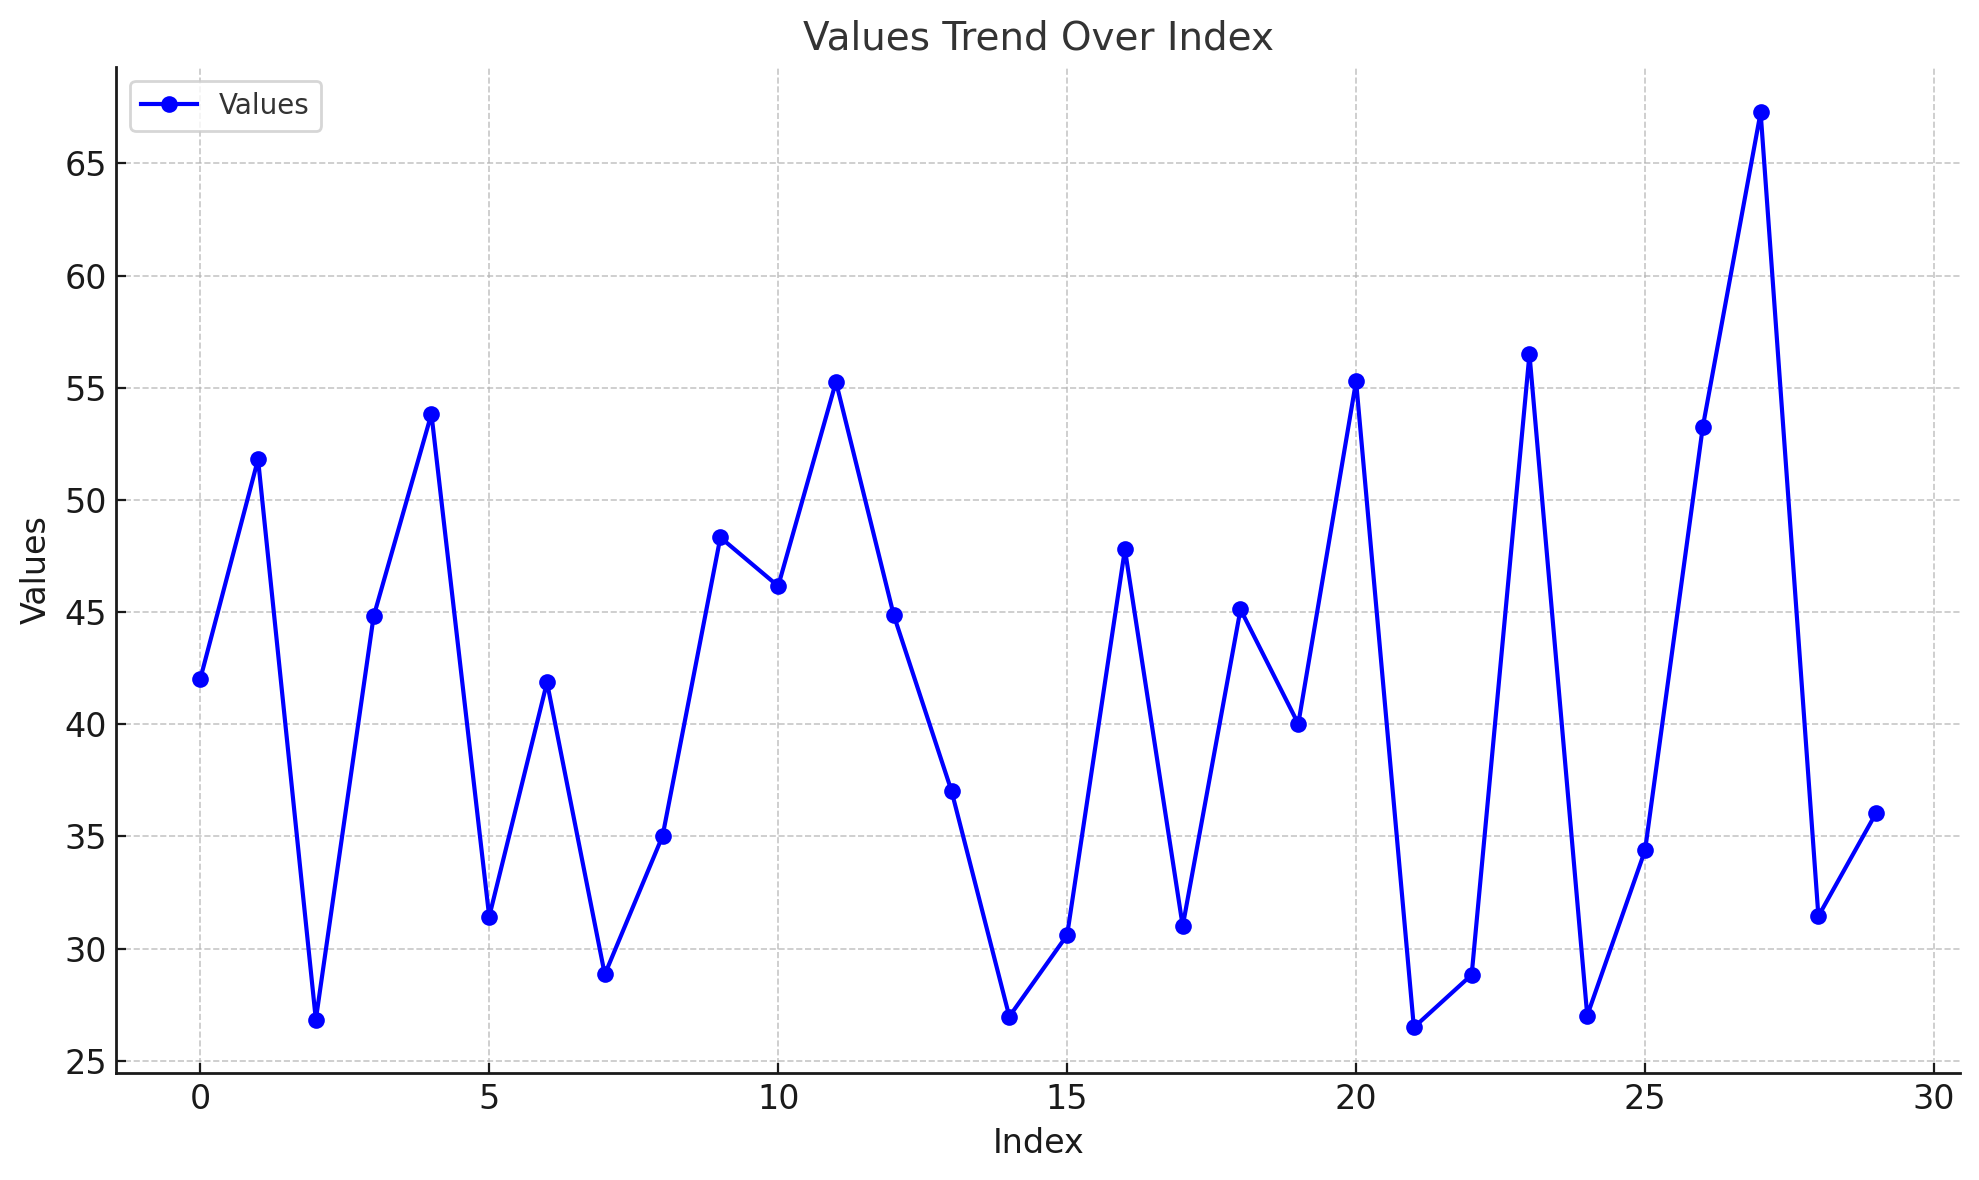
\includegraphics[width=0.6\linewidth]{../data/plot/trend_values_basic.png}
	\caption{Mutliple run reward - REINFORCE with no baseline}
	\label{fig:plot15}
\end{figure}

\subsubsection{More epochs}
To gain deeper insights into the methods, the number of epochs was increased, but the overall results remained consistent. Variability persists across the runs.

When training is extended to more epochs, the first two methods show slight improvements, while the third method (normalized rewards) remains unchanged. Specifically, the basic method achieves an average reward of 37.30 after a training time of 57 seconds, the constant baseline improves to 123.60 with a training time of 186.42 seconds, and the normalized rewards method achieves 53.03 with a training time of 112.28 seconds.

In testing, increasing the number of epochs yields higher rewards for the first two methods. The basic method improves 1.8 times to an average reward of 48.6, while the constant baseline sees a 2.1-fold improvement, reaching 276.9. However, the normalized rewards method remains largely unchanged, achieving a reward of 68.3, just a 1.02-fold increase.


\subsection{Actor-Critic Methods}
The two actor-critic methods, PPO (Figure \ref{fig:plot6}) and SAC (Figure \ref{fig:plot7}), were tested using the default values provided by the library, and their performance was compared over the same number of timestamps (50,000) The results revealed distinct behaviors between the methods. 

SAC demonstrates rapid learning during the initial phase, with a steep increase in rewards that plateaus around 30,000 timesteps. It achieves higher maximum rewards, stabilizing just below 450, but its progress slows significantly afterward. 

In contrast, PPO shows a slower start but maintains a consistent upward trajectory throughout the training, with rewards steadily increasing to approximately 350. Although PPO does not reach SAC’s peak performance, its consistent improvement highlights its stability and efficiency in training. Overall, SAC achieves higher rewards, but PPO offers more reliable and steady progress.

\subsubsection{Results}
The training times recorded highlighted significant differences between the actor critic methods. SAC required an average of 299.40 seconds per training run, whereas PPO completed training in an average of 14.89 seconds. This indicates that SAC is approximately 20 times slower than PPO. 

At first glance, the graphs might suggest that SAC could achieve better results, but this is not the case. SAC is slower due to the additional computations required during training and tends to overfit to the specific seed, limiting its ability to fully generalize. As a result, SAC occasionally fails to achieve the optimal outcome.

In contrast, PPO consistently achieves a perfect score over 300 episodes, with a performance of $ 500 \pm 0.0 $, compared to SAC’s $495 \pm 27$. Despite this slight difference, both methods deliver exceptional results, especially when compared to the performance of reinforce algorithms.

\begin{figure}[h]
	\centering
	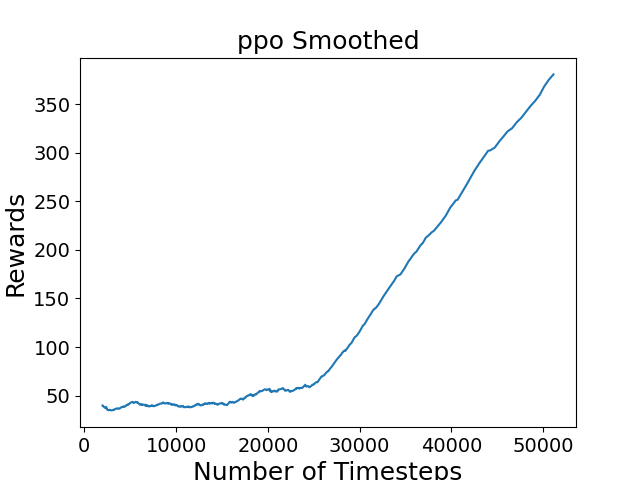
\includegraphics[width=0.5\linewidth]{../data/plot/ppo_ContinuousCartPole-v0_50k.png}
	\caption{Reward history - PPO}
	\label{fig:plot6}
\end{figure}


\begin{figure}[h]
	\centering
	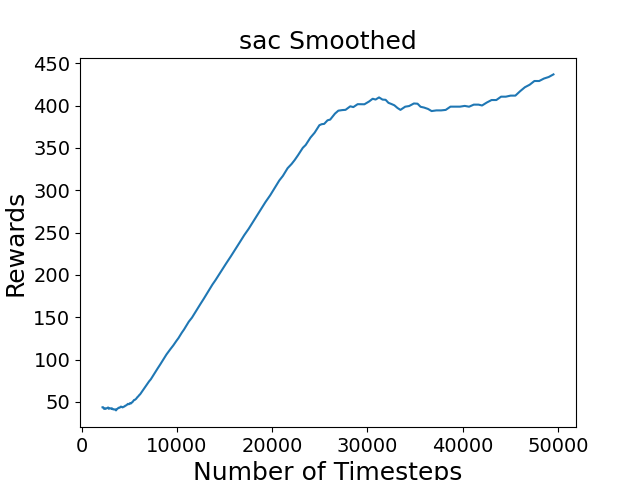
\includegraphics[width=0.5\linewidth]{../data/plot/sac_ContinuousCartPole-v0_50k.png}
	\caption{Reward history - SAC}
	\label{fig:plot7}
\end{figure}

\newpage

\section{Conclusion}
For continuous state and action spaces, SAC and PPO are generally the top choices, with PPO often holding a slight advantage. PPO is faster to train and consistently achieves a perfect score during testing. While SAC requires longer training and performs slightly worse, it still delivers excellent results overall.

Conversely, the reinforce algorithm demonstrates lower efficiency in achieving the goal across all the methods analyzed. Among the tested approaches, the method using a constant baseline performs the best, followed by the normalized rewards method, while the basic version consistently lags behind in both the number of epochs tested.

The basic reinforce algorithm uses Monte Carlo sampling to estimate returns, therefore the variance grows with the trajectory length. For continuous actions, this variance problem becomes even more pronounced because the action space is infinite, making it harder to get good samples that represent the action distribution well.

Adding a constant baseline helps reduce variance somewhat by subtracting an average value from the returns. However, in continuous spaces, a constant baseline is often too simple to capture the complexity of the value function. While it's better than basic REINFORCE, it still tends to have stability issues with continuous actions.

Normalizing rewards helps address the scale problem by keeping rewards in a consistent range, which can make learning more stable. However, like the constant baseline approach, this alone doesn't solve the fundamental variance issues of REINFORCE in continuous spaces.



%===============================================================================

%===============================================================================

%===============================================================================

% no \bibliographystyle is required, since the corl style is automatically used.
\bibliography{example}  % .bib

\end{document}
